\documentclass[draft,ms]{agutexSI2019}

\usepackage{graphicx}
\usepackage{amsmath}
\usepackage{amssymb}
\usepackage{mathtools}
\usepackage{rnn}
\usepackage[capitalise,noabbrev]{cleveref}

\newcommand{\citep}{\cite}
%
%  Uncomment the following command to allow illustrations to print
%   when using Draft:
\setkeys{Gin}{draft=false}
%
% You may need to use one of these options for graphicx depending on the driver program you are using.
%
% [xdvi], [dvipdf], [dvipsone], [dviwindo], [emtex], [dviwin],
% [pctexps],  [pctexwin],  [pctexhp],  [pctex32], [truetex], [tcidvi],
% [oztex], [textures]
%
%
%% ------------------------------------------------------------------------ %%
%
%  ENTER PREAMBLE
%

%% ------------------------------------------------------------------------ %%


% Author names in capital letters:
\authorrunninghead{SMITH ET AL.}

% Shorter version of title entered in capital letters:
\titlerunninghead{TEMPORAL SUBSAMPLING DIMINISHES SMALL SCALES IN RNNS FOR GFD}

%Corresponding author mailing address and e-mail address:
\authoraddr{Corresponding author: T. A. Smith,
(tim.smith@noaa.gov)}

\begin{document}

%% ------------------------------------------------------------------------ %%
%
%  TITLE
%
%% ------------------------------------------------------------------------ %%

%\includegraphics{agu_pubart-white_reduced.eps}


\title{Supporting Information for ``Temporal Subsampling Diminishes Small Spatial Scales in
    Recurrent Neural Network Emulators of
    Geophysical Turbulence''}

\authors{
Timothy A. Smith\affil{1,2},
Stephen G. Penny\affil{1,3},
Jason A. Platt\affil{4},
Tse-Chun Chen\affil{5}
}
\affiliation{1}{Cooperative Institute for Research in Environmental Sciences
    (CIRES) at the University of Colorado Boulder, Boulder, CO, USA
}
\affiliation{2}{Physical Sciences Laboratory (PSL), National Oceanic and
    Atmospheric Administration (NOAA), Boulder, CO, USA
}
\affiliation{3}{Sofar Ocean, San Francisco, CA, USA}
\affiliation{4}{University of California San Diego (UCSD), La Jolla, CA, USA}
\affiliation{5}{Pacific Northwest National Laboratory, Richland, WA, USA }

\begin{article}

%% ------------------------------------------------------------------------ %%
%
%  TEXT
%
%% ------------------------------------------------------------------------ %%


\noindent\textbf{Contents of this file}
\begin{enumerate}
    \item Figure S1
    \item Sensitivity to Activation Function
    \item Figures S2-S4
\end{enumerate}
\end{article}
\clearpage

\begin{figure}
    \centering
    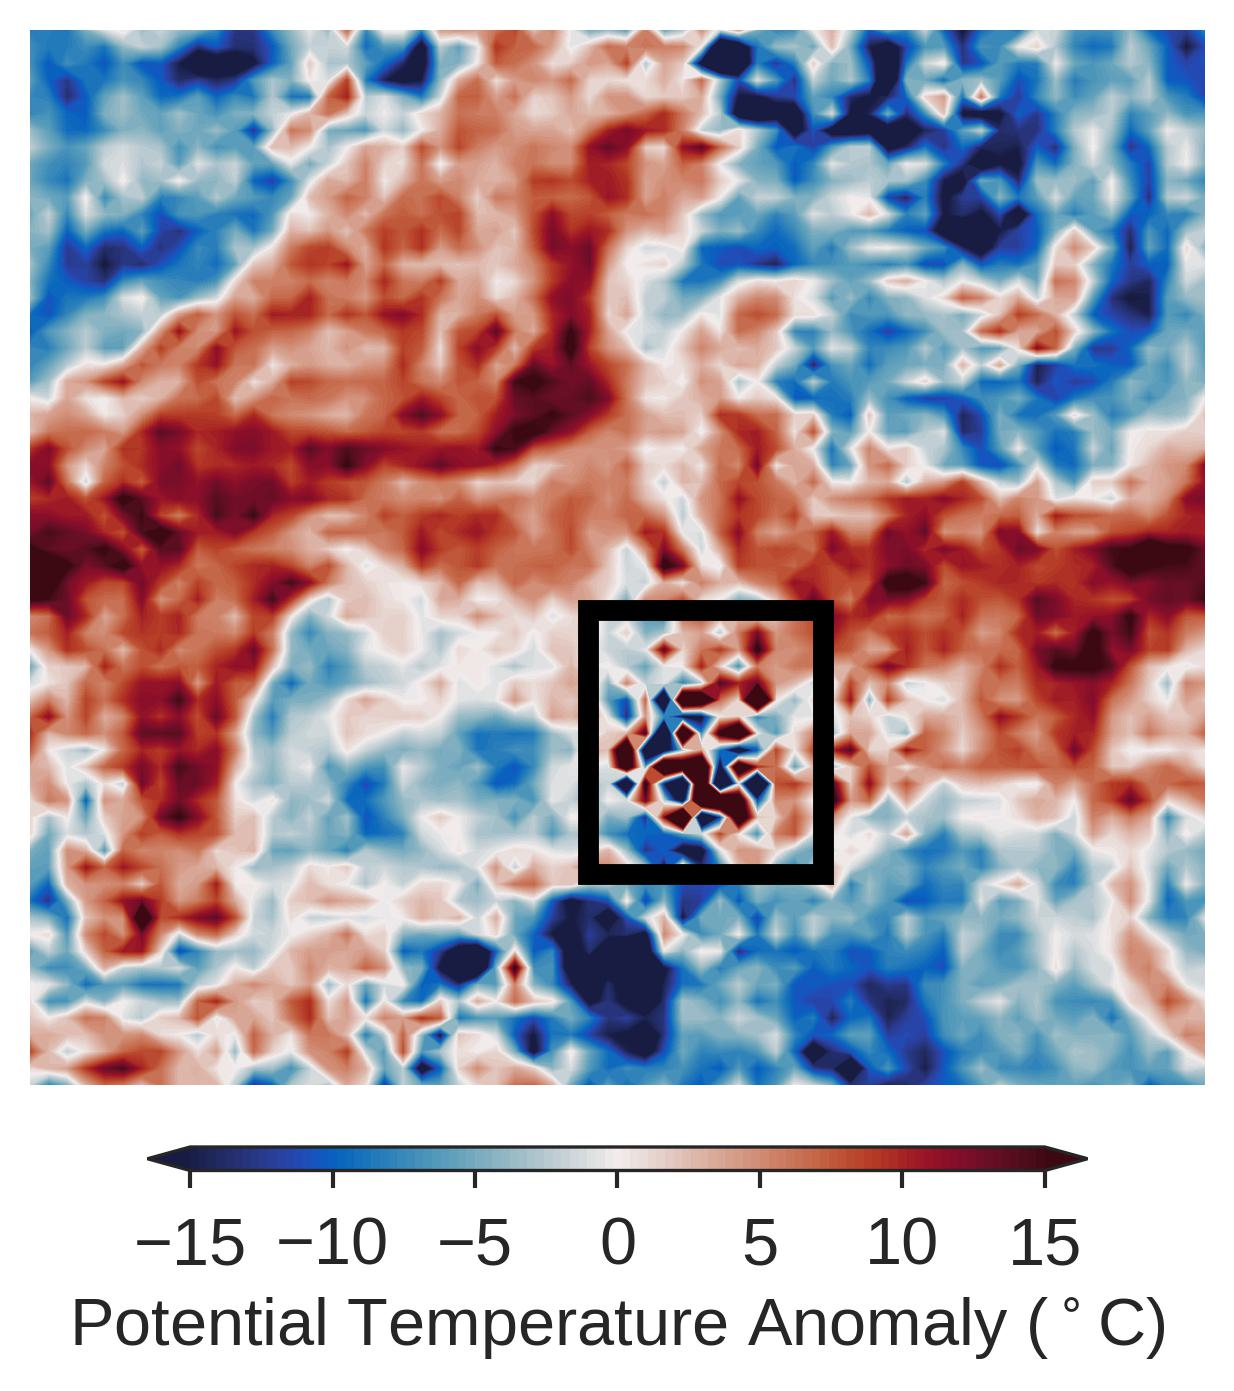
\includegraphics[width=.3\textwidth]{figures/nvar_instabilities.jpg}
    \caption{A view of the numerical instabilities generated by the NVAR model.
        The instabilities manifest as spiking oscillations, which are
        especially strong in the black box.
        This particular example occurs after 8~hours, given the same initial
        conditions in Figure 4 and $\nsub$~=~1, $\nlag$~=~1.
    }
    \label{fig:nvar_instabilities}
\end{figure}

\section*{Sensitivity to Activation Function}

In light of the work by \citet{sitzmann_implicit_2020}, we test the impact of
using a periodic sine activation function, including the initialization
scheme outlined by \citet{sitzmann_implicit_2020}.
We compare its performance to the standard tanh function.
The results shown here were produced by repeating the analysis shown in
Section 5 of the main manuscript, including the parameter optimization
procedure, with a sine activation function.

\cref{fig:tanh-vs-sine-qual,fig:tanh-vs-sine-quant} show a qualitative and
quantitative view of the comparison between using a tanh and sine activation
function.
The middle panel of \cref{fig:tanh-vs-sine-quant} shows that the sine activation
function can achieve much lower KE\_NRMSE and this is the case for
$\nsub=\{1,4\}$.
In fact, using a sine activation function results in the first model that
is competitive with persistence in terms of KE\_NRMSE
(\cref{fig:tanh-vs-sine-quant}, middle panel, $\nsub=1$).
The far right panel of \cref{fig:tanh-vs-sine-quant} shows that the lower error
incurred with a sine function instead of tanh is indeed due to better
representation of the small scale features.



\begin{figure}
    \centering
    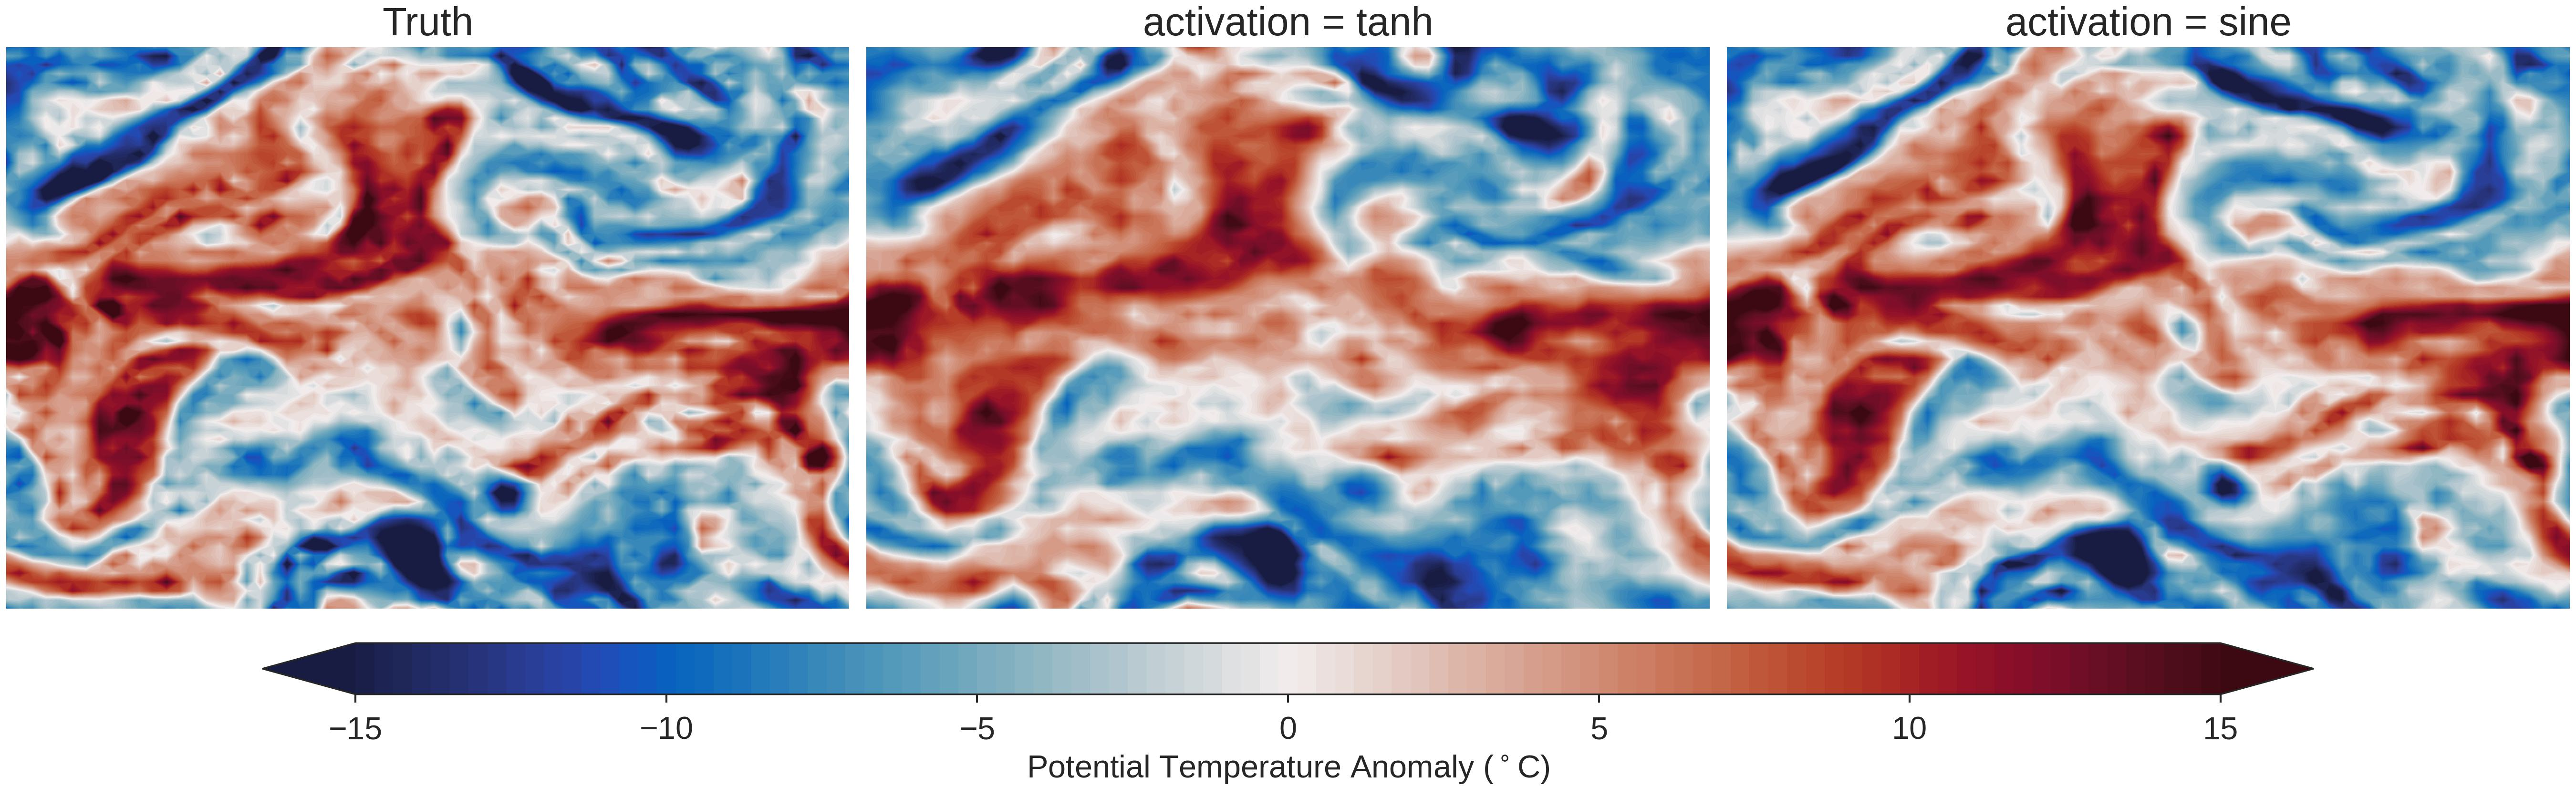
\includegraphics[width=\textwidth]{figures/rc_tanh_vs_sine_qualitative.jpg}
    \caption{
        One sample prediction from the test dataset with ESN models, comparing the use of
        tanh and sine activation functions. Here $\nsub = 4$ and $\gamma =
        10^{-2}$ in
        Equation (12). Each panel shows the prediction at a forecast lead time
        of 4~hours, using the same initial conditions as in Figure~4.
    }
    \label{fig:tanh-vs-sine-qual}
\end{figure}

\begin{figure}
    \centering
    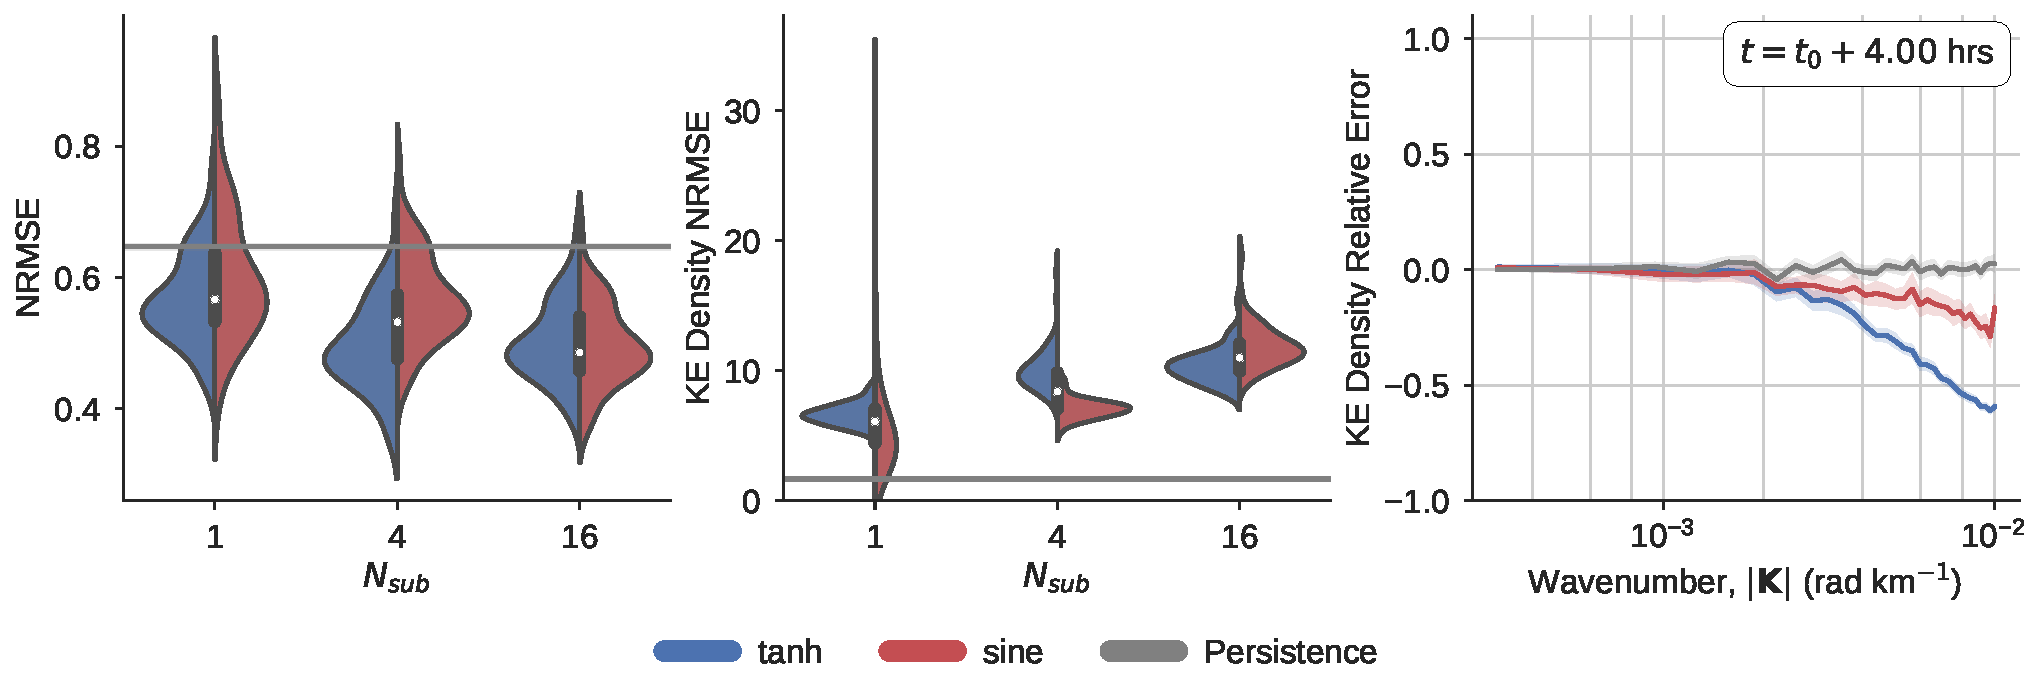
\includegraphics[width=\textwidth]{figures/rc_tanh_vs_sine_quantitative.pdf}
    \caption{
        Quantitative comparison of ESN predictions, comparing the using of
        tanh and sine activation functions. Here
        $\gamma = 10^{-2}$ in Equation (12).
        The sine activation outperforms tanh for $\nsub=\{1,4\}$ in terms of
        spectral errors, but does not for $\nsub=16$. The right panel shows the KE
        relative error at 4~hours for $\nsub = 1$ to show the scales at which error
        occurs.
    }
    \label{fig:tanh-vs-sine-quant}
\end{figure}

However, the representation of the small spatial scales is quite poor unless
they are prioritized in some way, as we do with a KE\_NRMSE term in the cost
function.
\cref{fig:sine-gamma} shows prediction skill comparing the case where the
KE\_NRMSE penalty is turned off ($\gamma=0$; blue) and when it is turned on
($\gamma=10^{-2}$; red).
The middle and right panels of \cref{fig:sine-gamma} show that prioritizing
small spatial scales in the loss function is required to accurately represent
them in predictions.

Moreover, even when the spectral penalty is turned on, temporal subsampling
results in diminished small spatial scales.
The red violin plots in the middle panel of \cref{fig:sine-gamma} show a gradual
increase in error as the data are further subsampled.

\begin{figure}
    \centering
    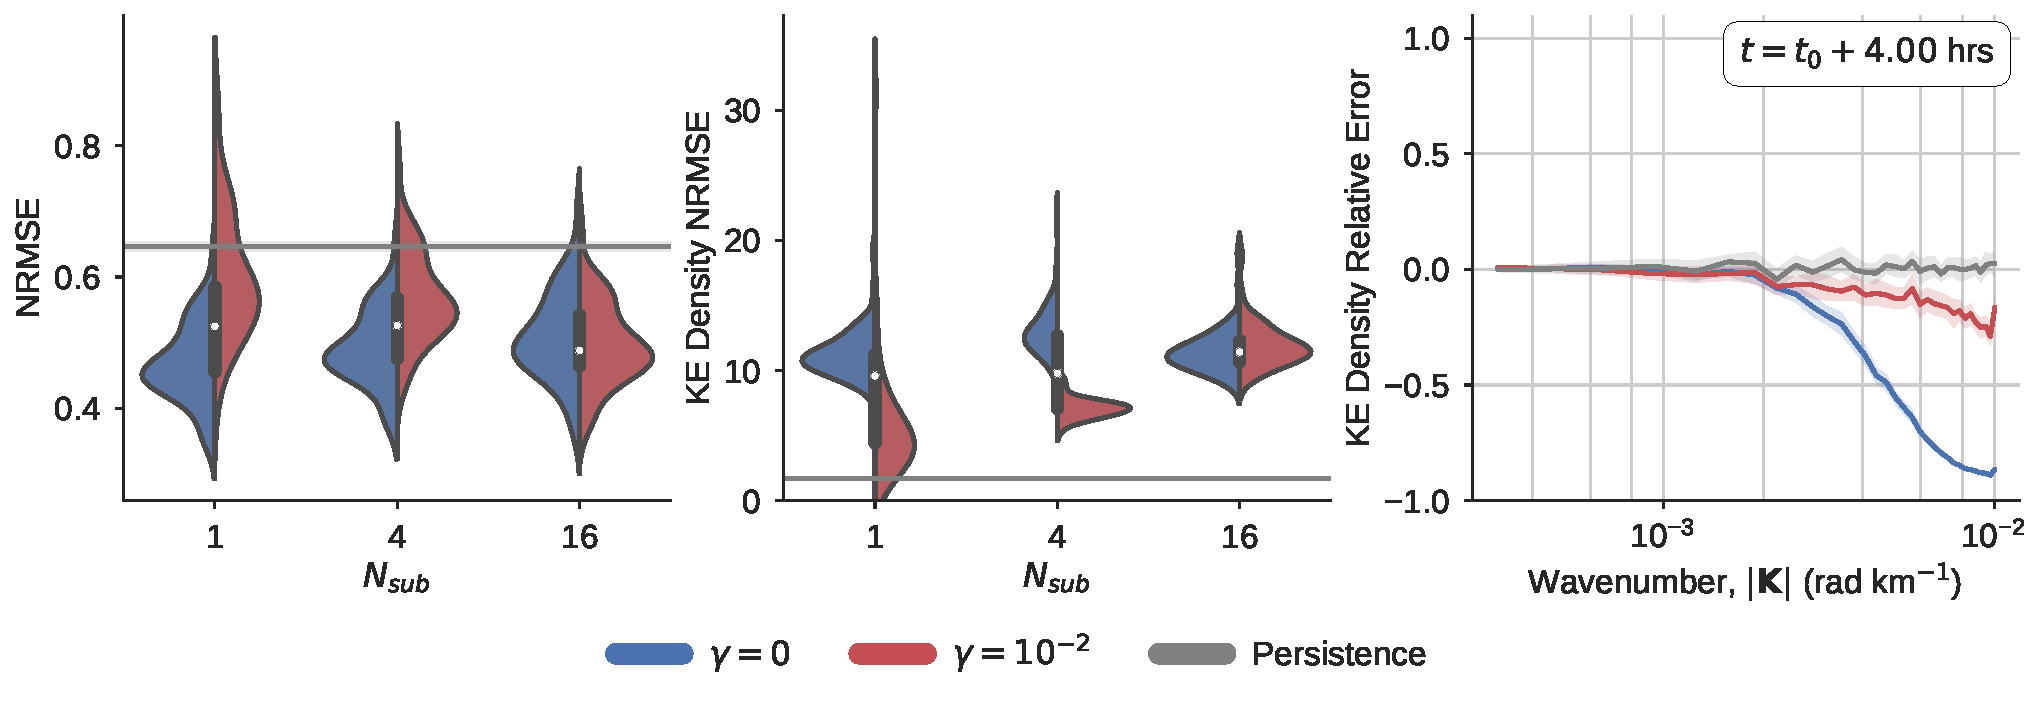
\includegraphics[width=\textwidth]{figures/rc_sine_gamma_quantitative.pdf}
    \caption{
        Quantitative comparison similar to \cref{fig:tanh-vs-sine-quant}, except here the activation
        function is set to sine in all cases, and the colors indicate whether KE\_RMSE is
        included in the parameter optimization or not by the amplitude of
        $\gamma$. The
        right panel shows KE relative error at 4 hours for $\nsub = 1$.
    }
    \label{fig:sine-gamma}
\end{figure}

\bibliography{references.bib}
\end{document}

